In our day-to-day lives, we constantly use our hands to hold, operate and otherwise manipulate objects, tools and devices with precision. We use them to gather tactile information about the world and even to communicate with each other through hand gestures and body language. They are a fundamental part of the human body and our way of interacting with the world around us.

The biggest buzzword's in the Virtual Reality (VR) medium: immersion and presence, perhaps point us in the right direction. VR is meant to bring us closer than ever before to experiencing virtual environments as if we were actually in them. Interaction is a big part of experiencing the places we are in. It should hardly be a point of contention then, that having virtual hands that imitate our own real hands can have a significant impact on VR experiences.

VR game developers and hardware manufactures alike have acknowledged this. Major consumer-oriented VR devices like the HTC Vive, the PlayStation VR  with the PlayStation Move Motion Controllers (PS VR + Move) and the Oculus Rift + Touch have controllers that track the position of your hands in space \parencite{htcvive2016, psvr2016, psmove2010, oculus2016}. In their About page, Owlchemy Labs, the creators of the critically and commercially acclaimed \parencite{UnityAwards2016, SteamSpyJobSim} Job Simulator: the 2050 archives \parencite{OwlchemyLabs2016} declare:

\begin{displayquote}
\textit{We believe that interaction and using your hands is what truly makes virtual reality the most incredible place to build unique content that blows players minds.} \parencite{aboutOwlchemyLabs}
\end{displayquote}

Predictably enough, this is not the end of the story. Even if we had complete tracking of the hands and individual fingers, the physical constraints of the virtual environment would still not apply to the users' real hands, which leaves us with few essentially different options:

\begin{enumerate}
\item Prioritize user input and ignore virtual environment constraints whenever there is a conflict in order to always keep the virtual hands aligned with the real hands to the extent allowed by the tracking data.
\item Separate the virtual hands from the real hands when there is conflict in order to respect the virtual environment's constraints.
\item Use sensory feedback that makes the users either respect the virtual constraints on their own or feel like they are constrained without actually being so.
\item As \parencite{Schell2015} suggests, design in a way that circumvents the problem, which means restricting the medium's content to experiences that fit exactly to the medium's current affordances \parencite{Norman}. This means seeing limitations as features and finding experiences that map perfectly to the current systems.
\end{enumerate}

The work here presented is focused on the second option, which is seen as a directly opposite alternative to the first. We aim to explore how virtual hands can work in this case and investigate whether the user experience can be improved with this approach.

From this point on, we will refer to this problem as the virtual world constraints problem, to the first option as unadjusted hand control model and to the second option as adjusted hand control model.

\section{State of the Art}
\label{sec:stateOfTheArt}

\subsection{VR Hardware}
\label{subsec:vrHardware}

There is a considerable amount of devices and accesories that are relevant to VR. This work is mainly applicable to those setups that can spatially track the hands of the user to a similar or greater degree than the HTC Vive allows. We are particularly interested in findings that are relevant to the aforementioned HTC Vive, PS VR + Move and the Oculus Rift + Touch because they are currently the most important consumer-oriented devices with these capabilities \parencite{Armstrong2017, SuperDataLLC2017}.

\begin{figure}[h]
\centering
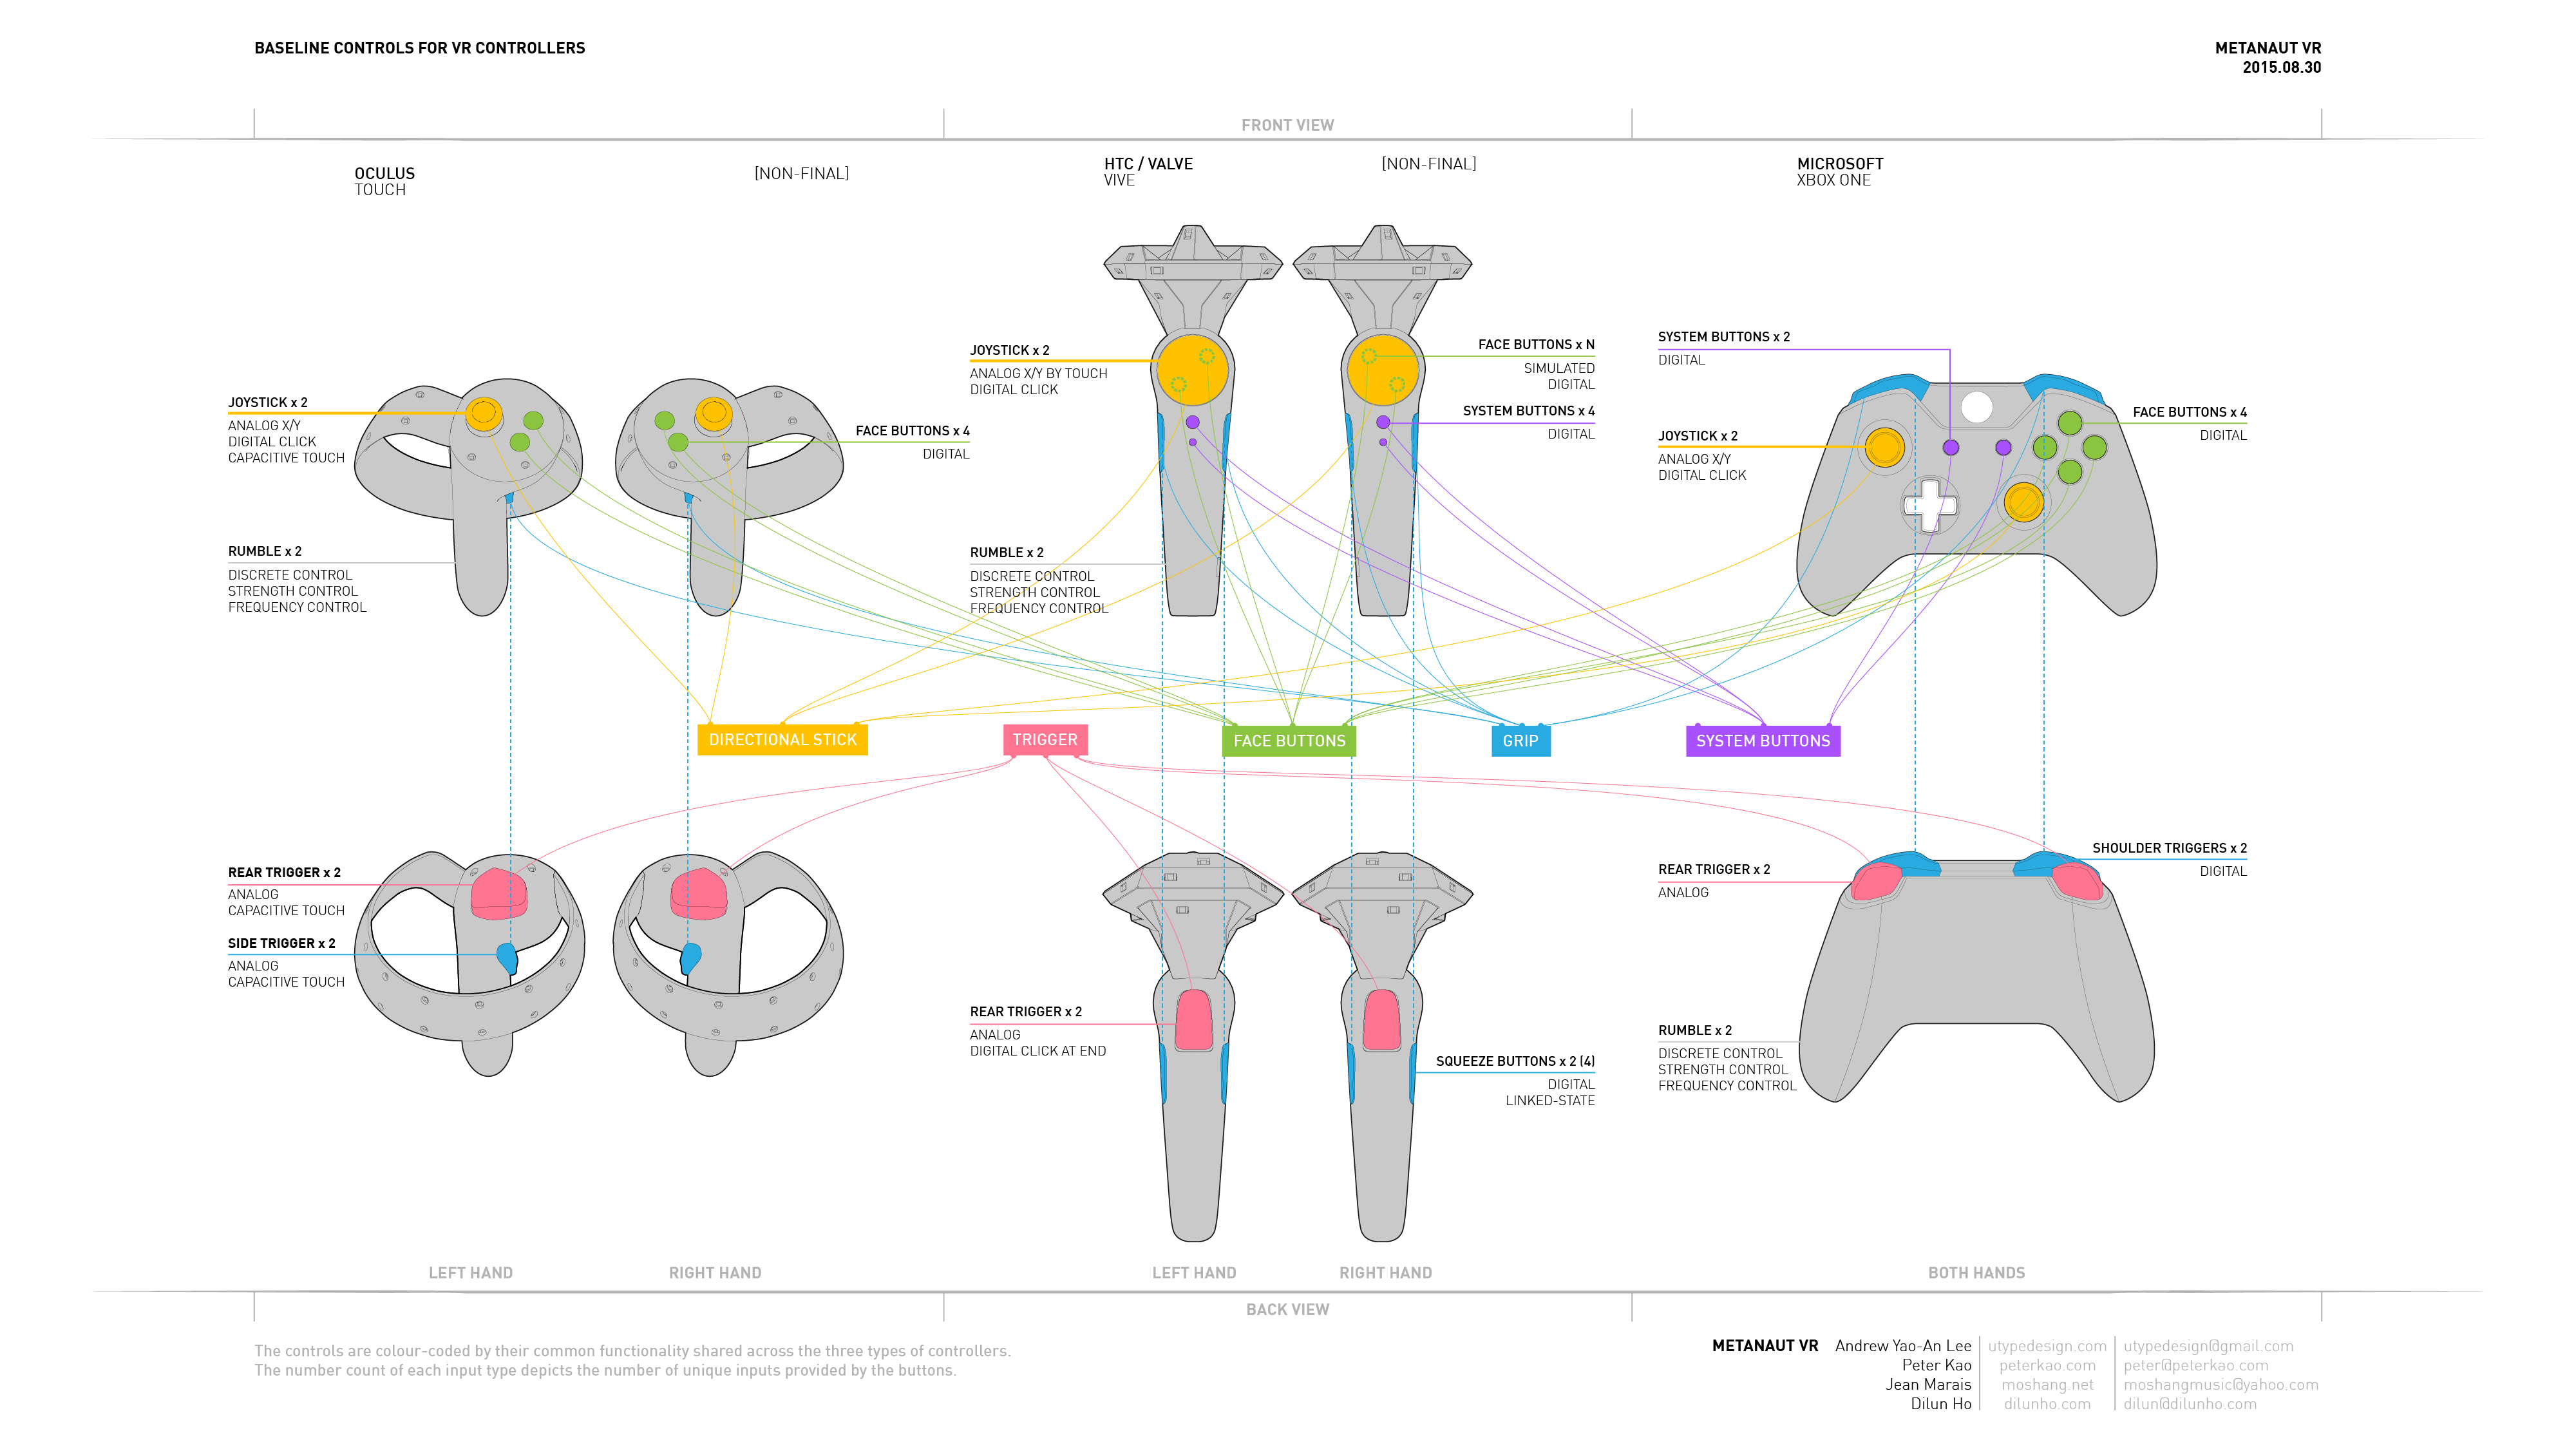
\includegraphics[width=\textwidth]{vrcontrollersbaselinecomparison2c.png}
\caption{Comparison of VR controllers and their different input and output capabilities. Retrieved from\parencite{MetanautVR2015}.}
\label{fig:vrControllerComparison}
\end{figure}

There are differences between the Head Mounted Displays (HMD) of these devices, but for the most part, they are not relevant for our area of focus, so they will not be discussed here.

On the other hand, it might be worth briefly covering the differences in terms of spacial tracking of the controllers between the devices. The HTC Vive allows 360 degree tracking within the biggest space volume, the Oculus Rift + Touch with the default setup is designed mainly for 180 degree tracking, but an experimental setup with extra components allows stable 360 tracking \parencite{Lang2016, Kuchera2016}.

Figure \ref{fig:vrControllerComparison} shows the features of the Oculus Touch and the HTC Vive controllers. In the case of the HTC Vive, the most relevant features for our purposes are:

\begin{itemize}
\item the analogue triggers with digital click at the end, controlled with the index finger, 
\item the digital grip buttons, pressed with middle, ring and/or pinky fingers,
\item the joysticks or trackpads, with analog x/y input through capacitive touch and digital click, used with the thumbs
\item and rumble capabilities (discrete, strength, frequency).
\end{itemize}

In the case of the Oculus Touch, the relevant features are:

\begin{itemize}
\item the analogue triggers with capacitive touch, controlled with the index fingers, 
\item the analogue side triggers, pressed with middle, ring and/or pinky fingers,
\item the joysticks, with analog x/y input, digital click capacitive touch, used with the thumbs
\item and rumble capabilities (discrete, strength, frequency).
\end{itemize}

Figure \ref{fig:psmoveDiagram} shows the input mechanisms of the PS Move Motion Controller, again, the most relevant features are:

\begin{itemize}
\item the analogue T buttons, controlled with the index fingers,
\item several digital buttons controlled by the thumbs
\item and rumble capabilities.
\end{itemize}

\begin{figure}[h]
\centering
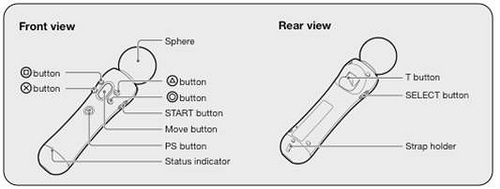
\includegraphics[width=\textwidth]{psmovecontroller.jpg}
\caption{Diagram of the PS Move Motion Controller. T button allows analogue input. Retrieved from \parencite{psmoveDiagram}.}
\label{fig:psmoveDiagram}
\end{figure}

Analogue buttons are useful to allow the users to control the motion of the virtual fingers with similar movements with their own fingers - in Norman's terms, they provide a natural mapping \parencite{Norman} for finger control. Similarly, although without the advantage of being analogue, buttons or areas with capacitive sensors can be used to monitor if the user's fingers are resting on the controller or are lifted, which can allow for guessing the position of the fingers. 

The Oculus Touch is the controller that takes these input mechanisms further having a capacitive trigger for the index finger, capacitive buttons for the thumb and a normal trigger for the other three fingers. This can be used to detect a variety of gestures like index finger pointing, thumbs up (or down), finger guns... It also facilitates common interactions like pressing virtual buttons with your virtual index finger, operating a grabbed object with the same hand that is holding it (e.g. press gun trigger). Both the HTC Vive and PS VR controllers allow for a lower degree of natural finger control.

Other accessories exist that allow for actual positional tracking of the fingers \parencite{ManusVR2016}. These would of course enhance the experience, but ultimately would face the same problem because they don't provide a way to impose constraints from the virtual world on the real hands of the user.

\subsection{VR Games}
\label{subsec:vrGames}

The most frequent approach to dealing with the virtual world constraints problem described at the beginning of this chapter is to ignore these constraints when they conflict with the user input. Job Simulator is a prime example of the unadjusted hand model and the one that we have used in our work as a baseline for comparison.

In Job Simulator the hands never separate from the position of the controller, but this still allows for reasonable physical interaction with small, light objects that can be easily moved by the hands. When the hands collide with movable objects, the object is pushed out of the way. However, when the virtual hands collide with objects that cannot be moved by them, the hands will simply go through them as if they weren't there as shown in Figure \ref{fig:jobSimStaticProblem}.

\begin{figure}[h]
\centering
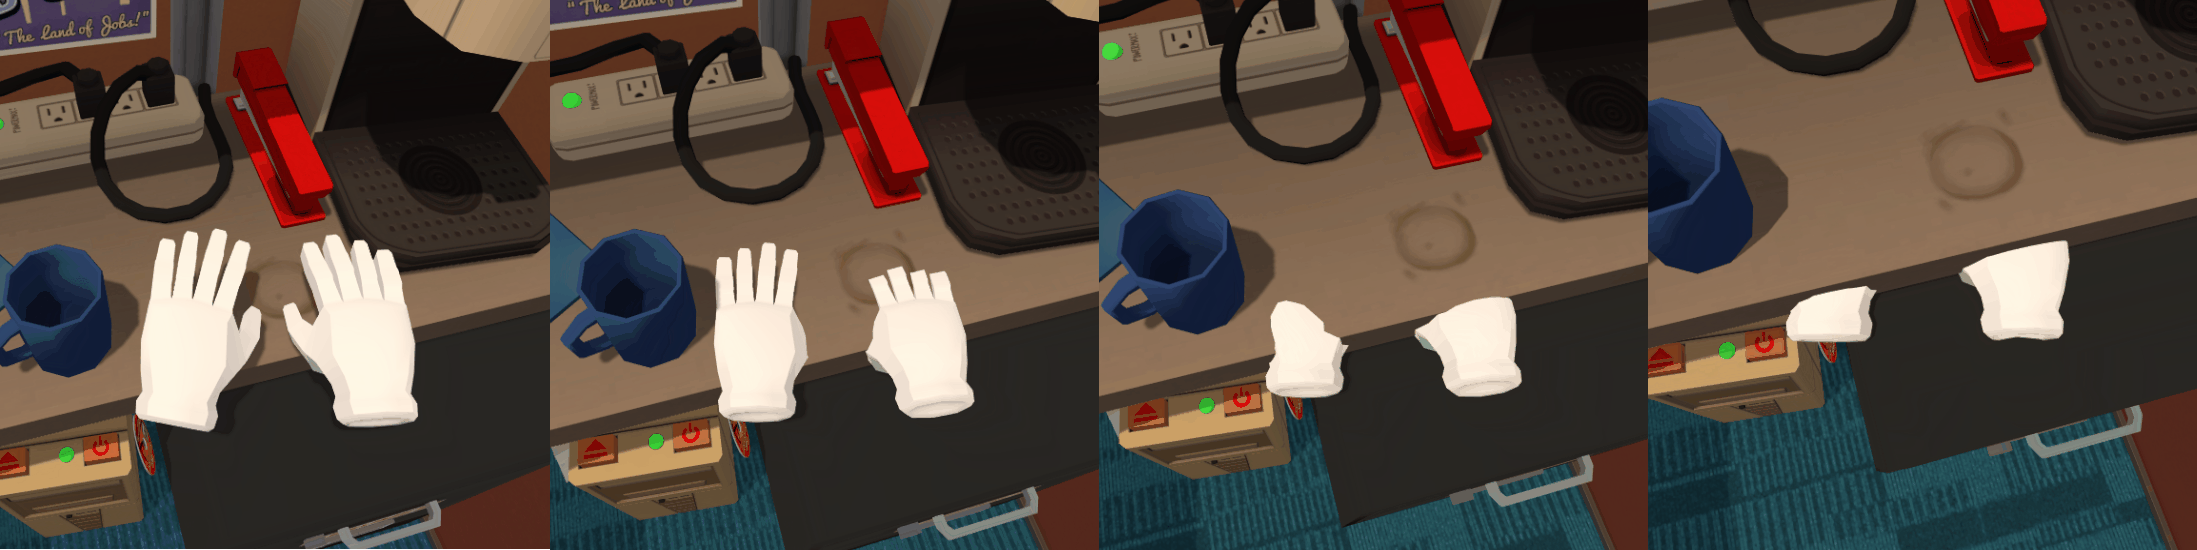
\includegraphics[width=\textwidth]{Sequences/JobSimulator/jomSimStaticProblem.png}
\caption{Sequence showing the Job Simulator hands entering an unmovable obstacle. Captured in the HTC Vive version.}
\label{fig:jobSimStaticProblem}
\end{figure}

At the same time, they avoid the problem of grabbing objects with correct finger placement by hiding the hands when they are holding an object as shown in Figure \ref{fig:jobSimGrabProblem}. This solution is not without merits: it allows the user to see the held object from all angles without the hand obstructing the view, it is simple and surprisingly, it is often not noticed by the users.

Ideally however, we would like the hand to be visible and the fingers to be correctly placed on the grabbed object forming a grip, but without adjusting the virtual hand, this requires the user to be too precise controlling the virtual hands and makes grabbing objects very difficult.

\begin{figure}[h]
\centering
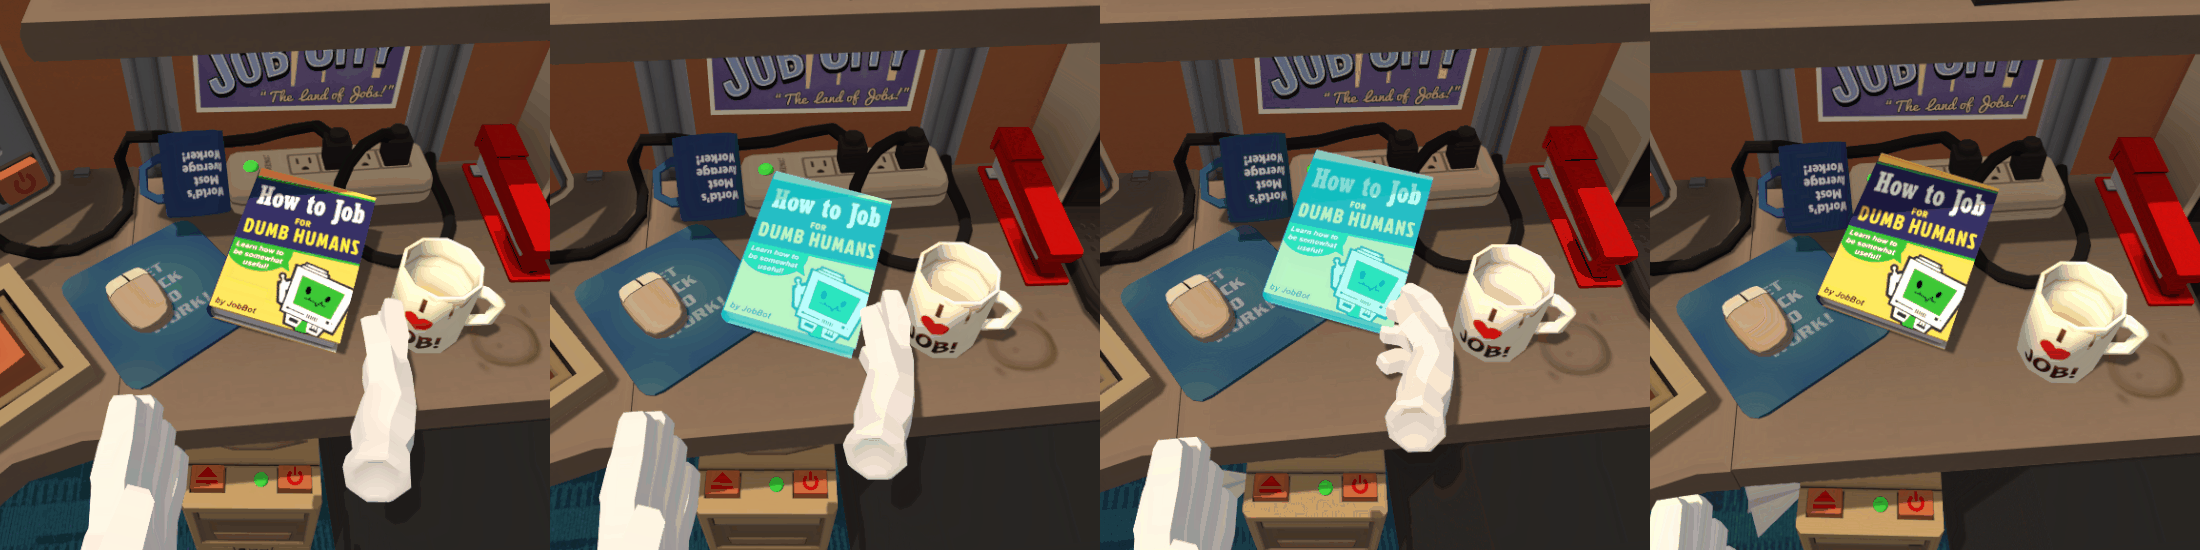
\includegraphics[width=\textwidth]{Sequences/JobSimulator/jomSimGrabProblem.png}
\caption{Sequence showing the Job Simulator hands grabbing an object. The hands are hidden while holding objects. Captured in the HTC Vive version.}
\label{fig:jobSimGrabProblem}
\end{figure}

Very recently, a few games have started to show approaches to hand control that fall within the adjusted hand model. One these is Wilson's Heart \parencite{TwistedPixelGames2017}, released in April this year. Each object that the user can interact with has a predefined hand pose and when certain conditions are met, the hands will snap to the pose as shown in Figure \ref{fig:wilsonGrab}. These conditions usually have to do with the user pressing some of the triggers or buttons that control the virtual fingers although there are also poses that are triggered by moving the hands close enough to the objects.

\begin{figure}[h]
\centering
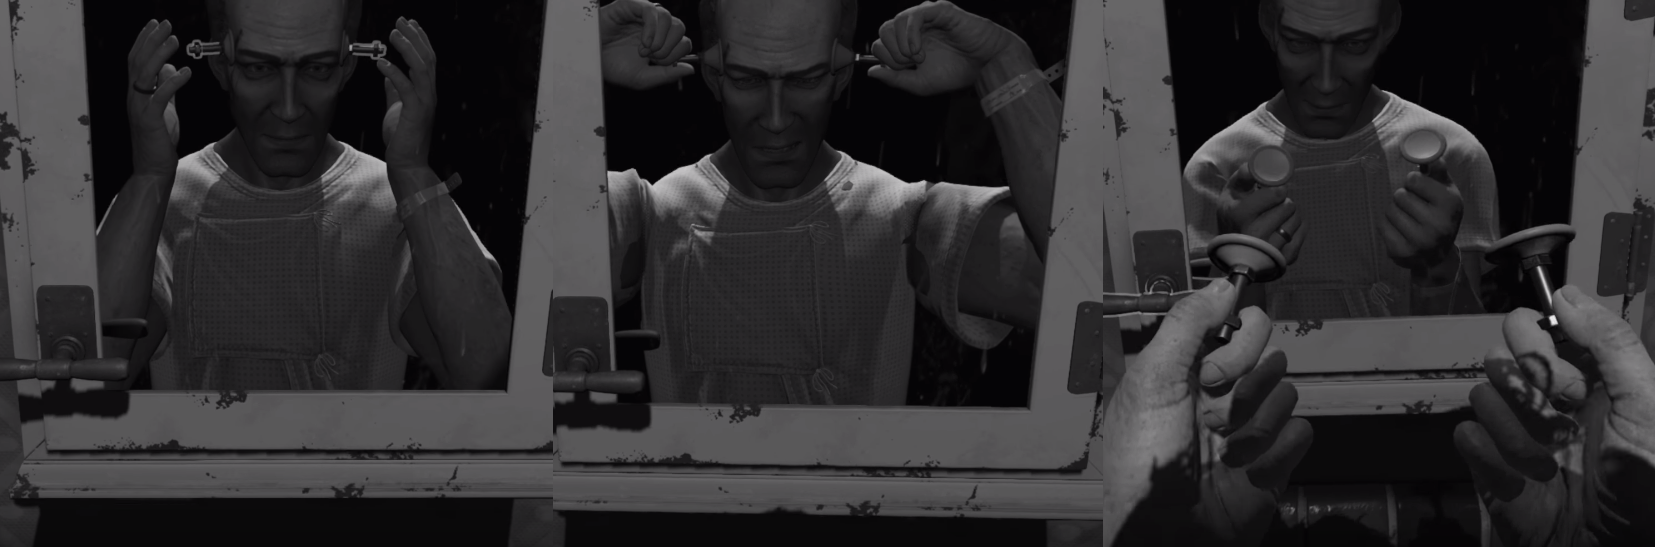
\includegraphics[width=\textwidth]{Sequences/WilsonsHeart/wilsonGrab.png}
\caption{Sequence showing the pose-snapping grab in Wilson's Heart.}
\label{fig:wilsonGrab}
\end{figure}

This technique is interesting because the virtual hands can separate a lot from the position of the real hands and very suddenly too. The underlying idea is that user's will want to interact with each object in a certain way and will on their own pose their hands in a similar way to the object's pose, so when the pose snapping happens, the change will be small and, most importantly, aligned with the user's intention. 

The pose-snapping method allows perfect placement of the fingers and looks great in pictures, but it requires a lot of manual work to setup every interactible object in the game and it takes away a lot of control from the users, forcing them to interact with each object exactly in the ways that the poses allow.

\begin{figure}[h]
\centering
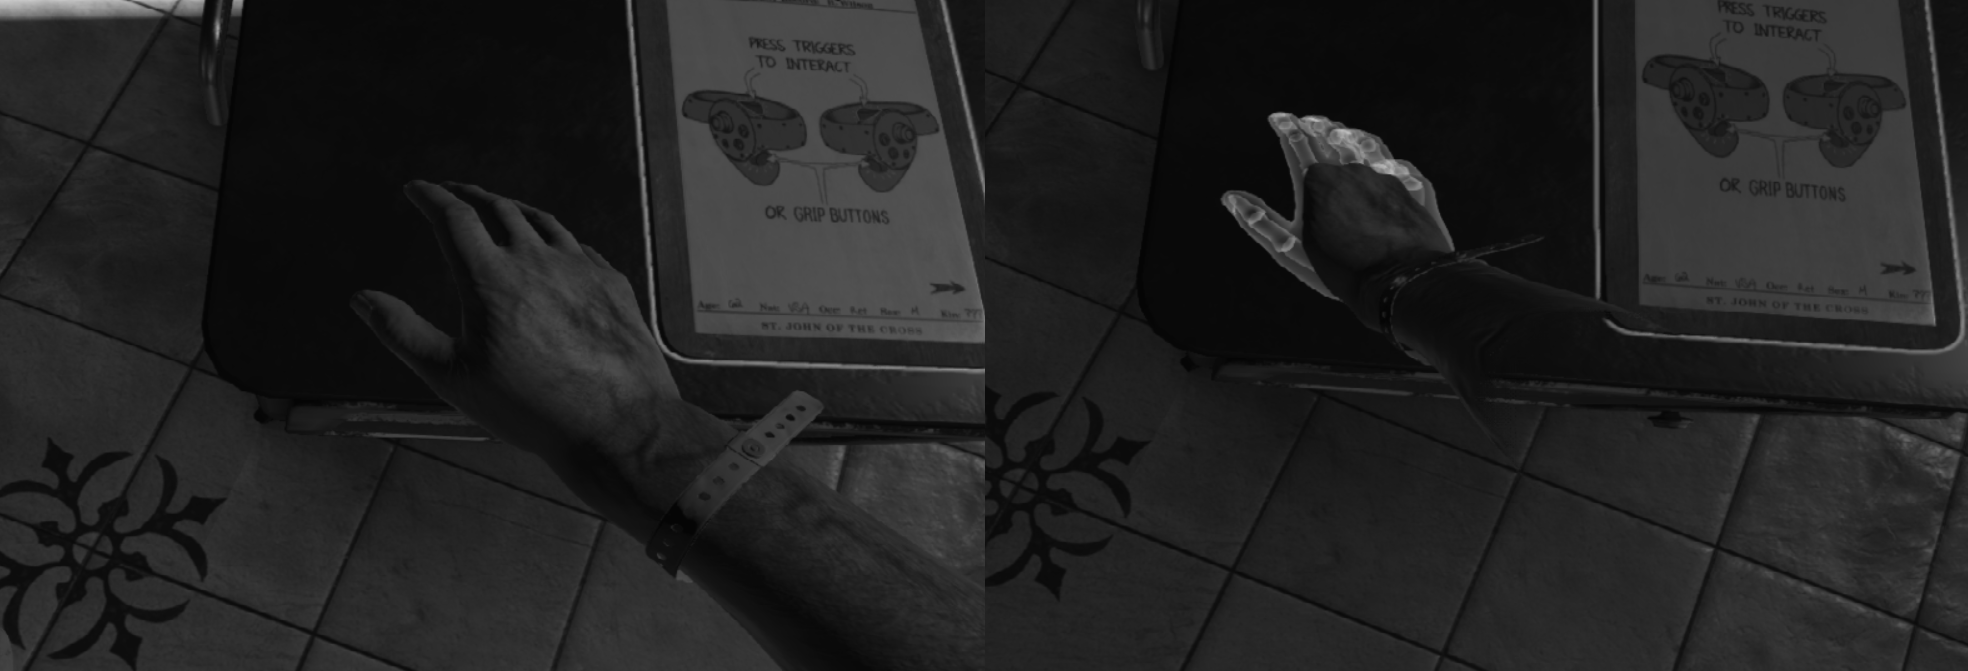
\includegraphics[width=\textwidth]{Sequences/WilsonsHeart/wilsonPenetration.png}
\caption{Sequence showing the the hands in Wilson's Heart entering an unmovable object. An X-Ray effect shows the part of the hand inside the object.}
\label{fig:wilsonPenetration}
\end{figure}

Figure \ref{fig:wilsonPenetration} shows that the other issue identified with the Job Simulator hands is mostly unsolved in Wilson's Heart. The hands can still go through unmovable objects, but in this case, an X-Ray style effect is used to visualize the parts of the hands that are inside of objects. This communicates the state of the hands to the player, but might not be preferable to other techniques that make the virtual hands respect the virtual world's physics.

The most novel and promising attempt within the adjusted hand model that we are aware of however, is an upcoming game called Lone Echo \parencite{ReadyAtDawn}. In this game, the virtual hands procedurally adapt to the virtual environment. Once again, the underlying principle is adjusting the virtual hand in a way that doesn't conflict with the user's intentions, but in this case instead of using authored poses the use of a real-time algorithm can make the system extremely flexible. At its best, this approach could empower the user and make them feel more control over their virtual hands by not forcing the interaction with objects to one specific pose. At its worse, there might be situations where the algorithm doesn't behave in a way that matches the user's natural way of interacting with their hands which would have the opposite effect.

This approach will inevitably come at the cost of having some edge cases that don't look as good authored poses, but in terms of development work, scales much better with the amount of objects in the virtual environment and these edge cases might be so rare that they barely impact the experience.

Figure \ref{fig:loneEchoGrip} tries to show the procedural hand posing shown in some of the available footage from the game, but in this case particularly - and in general for the other frame sequences included in this work - we encourage the reader to watch the linked videos and .gifs because a few frames can't possibly do them justice.

\begin{figure}[h]
\centering
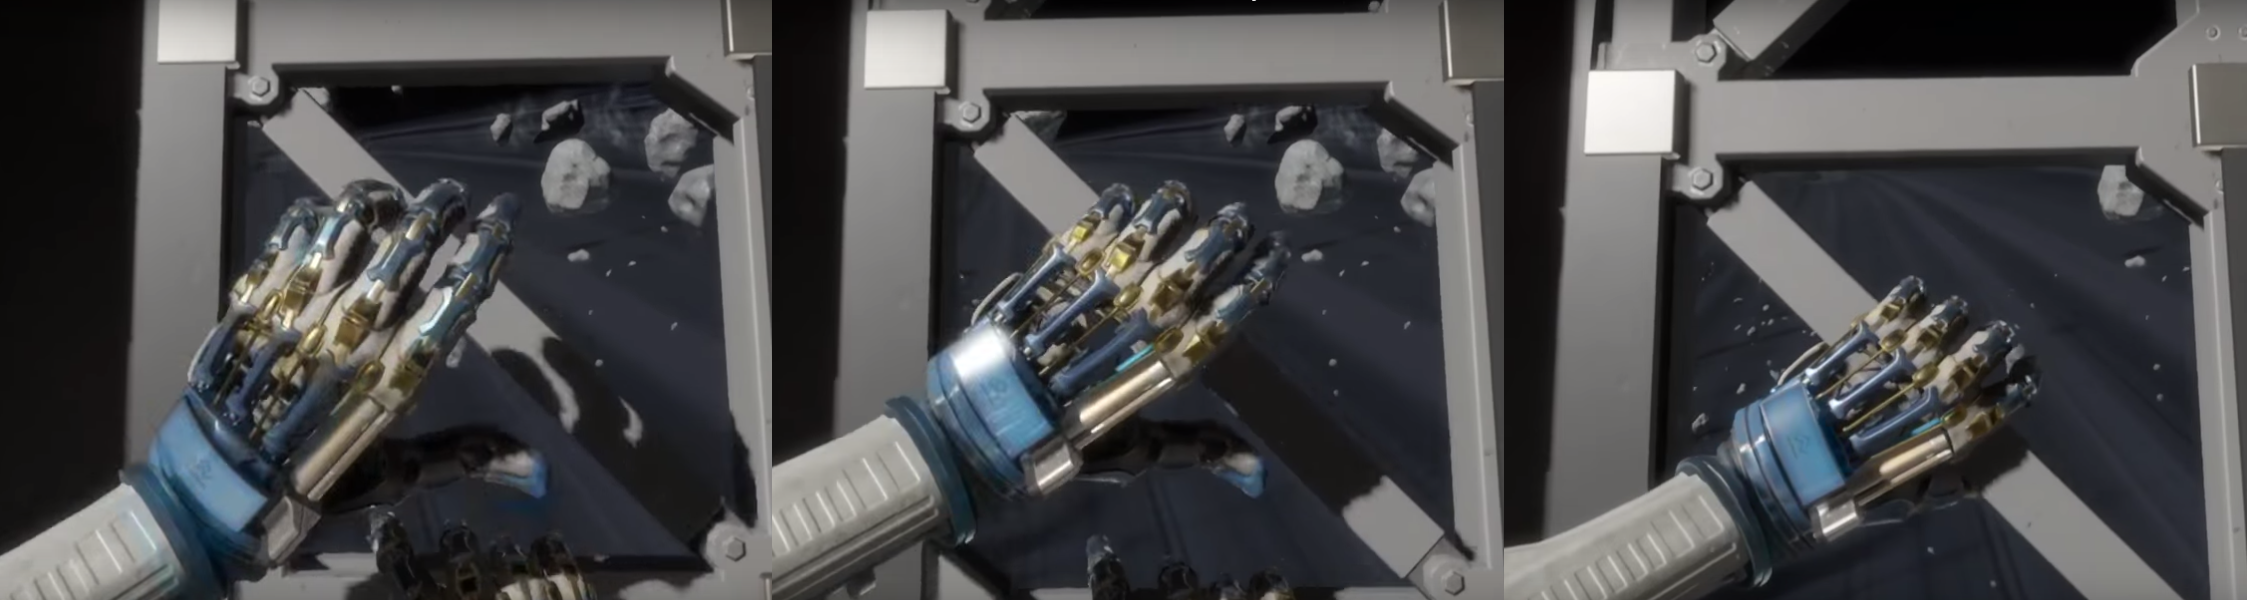
\includegraphics[width=\textwidth]{Sequences/LoneEcho/loneEchoGrip.png}
\caption{Sequence showing the procedural hand posing system in Lone Echo. Captured from video \parencite{loneEchoVideo}.}
\label{fig:loneEchoGrip}
\end{figure}

\section{Research Questions}
\label{sec:researchQuestions}

This work explores ways of dealing with the virtual world constraints problem previously described: how can we deal with the conflict between wanting the virtual hands to imitate the user's real hands and at the same time respect the virtual environment?

We see this problem manifesting itself specially prominently in two use cases:

\begin{enumerate}
\item The user places his real hand in a way that would make the corresponding virtual hand be inside of another virtual solid object.
\item The user wants to grab a virtual object but doesn't position the controller and otherwise produce the input that would in a strict simulation allow their virtual hand to lift the object.
\end{enumerate}

These properties should be pursued without losing the degree of control, consistency and intuitiveness that existing unadjusted hand models provide. In sum, the degree of "hand presence" (term commonly used in the VR industry \parencite{Bye2016}) achieved by this model cannot be lost in favor of these goals. The question this work addresses is whether "hand presence" can be improved by dealing with the virtual environment constraints problem.

As secondary objectives, we are interested in finding ways of conveying a sense of the weight of virtual objects when interacting with them and improving the tactility of the virtual hands, improving the feeling of touching virtual objects, which are also aspects currently unsatisfactorily addressed.

Therefore, we are trying to reduce the existing gap between the user's real body and their virtual body and compensate for imprecise user input. In terms of the user's perceptual, sensory experience, it might be possible to improve how hands are controlled in VR.

We focus on experimenting with different ways of adjusting the virtual hands' pose, exploring possible adjusted hand models. We will use the Job Simulator hand model, a great example of an unadjusted hand model, as a reference and baseline to compare our experiments with.